\chapter{Higgs decaying to two photons}

The Higgs to two photon channel is one of the most promising decays in the search for the SM higgs
at the LHC. Despite having a relatively small branching ratio, the decay $\Hgg$ 
provides a very clean, fully reconstructable final-state topology, making it 
one of the most sensitive channels at low mass.
The dominant source of background is from real, prompt diphoton events from QCD 
processes, $pp\rightarrow\gamma\gamma$.
In addition, there is a contribution from $pp\rightarrow\gamma+jet$ and $pp\rightarrow jet+jet$
in which jets are mis-identified as photons.
This chapter describes a search for a Higgs boson decaying to two photons
which was performed on the full 2011 dataset 
corresponding to \clumi of proton-proton collisions recorded at CMS at a center of mass energy of 7 TeV.

\section{Data samples}
\label{sec:datasamples}

The dataset used for this analysis is the combination of the 2011A and 2011B 
proton-proton collision runs.
The selection for the dataset used for this analysis is based around dedicated diphoton triggers
which select events online which satistfy one of two sets of criteria.
The first set requires two HLT photon candidates, one with $\pt>26$ GeV and the other with 
$\pt>18$ GeV, which are well isolated in the calorimeter. The second has a lower threshold on
the first photon, $\pt>22$ GeV but requires that both photons have localised showers in the ECAL 
($\rnine>0.8$ in 2011A and $\rnine>0.9$ in 2011B). 
Additionally, the invariant mass of the two trigger objects are required to have an 
invariant mass greater than 60 (70)GeV in the 2011A(B) datasets.
Events which would pass the full offline selection but failed to trigger at the HLT lead to an inefficiency, 
reducing the number of signal events with respect to that expected from an integrted luminosity of \clumi.
However, the tresholds applied offline are choson to be much tighter than those of the trigger;
the trigger efficiency is $>$99\% with respect to the analysis selection. 

Signal Monte Carlo (MC) events are generated for a Higgs decaying to two photons via the four main 
production processes, gluon-gluon fusion, vector boson fusion and assosiated $W/Z$ and $\ttbar$ production.
The gluon-gluon fusion (ggH) and vector boson fusion (qqH) were generated with \texttt{POWHEG} with 
next-to leading order (NLO) contributions whereas
the two associated production processes were generated to leading order (LO) only.
The $\pt$ spectrum of the Higgs ($\pt^{H}$) from gluon-gluon fusion was calculated at
next-to-next-to leading plus next-to leading log resummed order (NNLO+NLL) using the \texttt{HqT} program.
The production cross-sections and branching ratios are taken from the LHC Cross-section Working Group.

MC for background processes were generated at LO using \texttt{POWHEG} intefaced with \texttt{PYTHIA}.
The QCD dijet and $\gamma+jet$ samples are filtered by requiring the generated photons, electrons and neutral
mesons with $\pt>15$ GeV have at most one charged particle in a cone, $\Delta R<0.2$, to increase the 
production efficiency with respect to the tracker isolation requirements of the full selection.
The background samples considered for this analysis are summarized in Table~\ref{tab:backgroundmc}.
A full simulation of the CMS detector is provided in \texttt{GEANT4} which is used for all signal
and background MC samples.

\begin{table}
\begin{center}
\begin{tabular}{|l r|c|c|}
\hline
\textbf{Process}  & &  \textbf{Cross-section} ($pb$) & \textbf{Luminosity} ($pb^{-1}$)\\
\hline
\hline
DiPhotonJets & & 154.7 & 7400 \\
\hline
DiPhoton Box & $\hat{\pt}~25-250$ & 12.37 & 41900 \\
\hline 
QCD Dijet    & $\hat{\pt}~30-40$      & 10870 & 560 \\
	     & $\hat{\pt}~40-\infty$  & 43571 & 920 \\
\hline 
Gamma+Jet    & $\hat{\pt}~20-\infty$  & 493.44& 2400 \\
\hline 
DrellYan+Jets to $ll$  & $\hat{\pt}~50-\infty$  & 2475& 14000 \\
\hline
\end{tabular}
\caption{Background MC used throughput the analysis with production cross-sections and 
corresponding equivalent integrated luminsity.}
\label{tab:backgroundmc}
\end{center}
\end{table}


\section{Object Reconstruction and Identification}
\label{sec:objectrecoandid}

The reconstruction of all objects used in this analysis 
are based on the standardized reconstruction software available for all CMS analyses.
All data and MC samples are reconstructed with the standard reconstruction software \texttt{\cmssw}. 
Additional sensitivity can be gained by tayloring the object selection and reconstruction specifically
to the search for $\Hgg$. 


\subsection{Boosted Decision Trees}
General introduction about BDT's and what they do.
\label{sec:boosteddecisiontrees}


\subsection{Supercluster Energy Correction}
\label{superclusterenergyreconstruction}

As the natural width of Higgs boson is around 100 MeV, the width of a reconstructed mass peak from 
a $\Hgg$ decay is driven by the experimental energy resolution of the photons.
This resolution can be improved dramatically by correcting the raw energy of the supercluster 
on a per-photon level. These corrections are derived using a multivariate technique 
in which a regression BDT is trained on prompt photons in the gamma+jet MC sample using the 
ratio of the generated photon energy to the raw energy of the reconstructed supercluster.
As this ratio can vary across different regions of the detector, the input varibles include both the 
$\eta$ and $\phi$ positions of the supercluster. In addition, several variables are included which 
describe the shower shape: $\rnine$, the energy weighted widths in $\eta$ and $\phi$ of the supercluster,
the energy weighted crystal width ($\sigieie$) and the ratio of hadronic energy behind the supercluster
to the energy of the supercluster itself ($\hoe$). In the endcap, there is additional information 
available from the pre-shower. The ratio of the energy in the pre-shower to the raw supercluster energy
is included for superclusters in the ECAL endcap. Figure~\ref{fig:mcregrcomparisons} shows the improvement
in resolution after applying the regression corrections compared to the raw measurement.
In addition, a similar set of corrections were derived using by fitting an analytical expression 
of the residual energy difference between the 
generated and reconstructed photon energy as a functon of supercluster energy, position and $\rnine$. 
The regression technique reduces the effective resolution of the Higgs mass peak ($\sigma_{eff}$) 
resolution by around 30\% over using the raw supercluster energy compared to the analytic fit which
improves the resolution by 15\%. 

\begin{figure}
\begin{center}
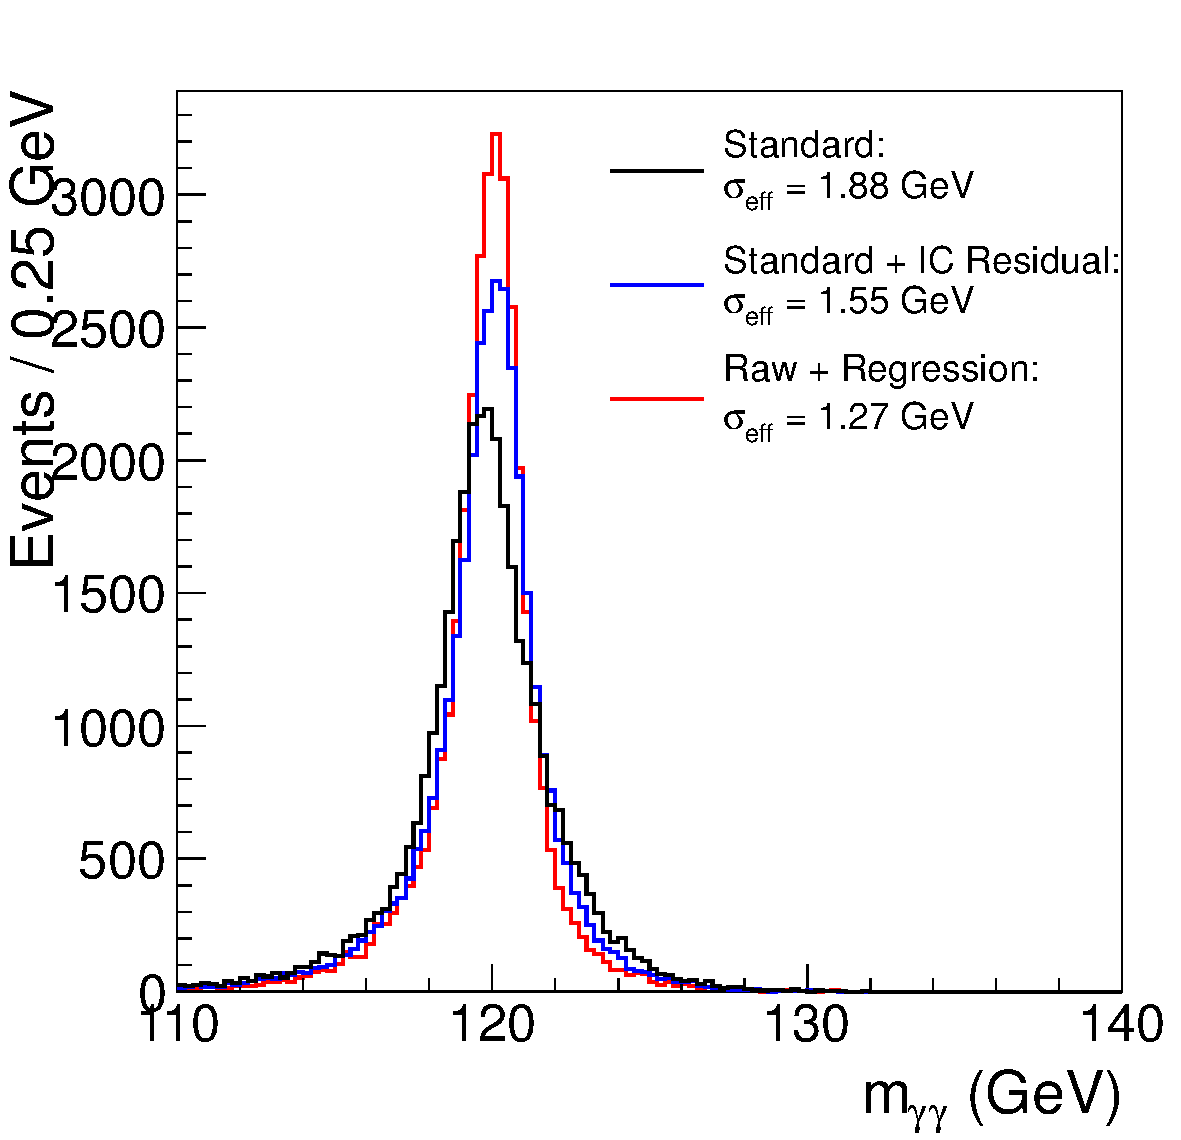
\includegraphics[width=.6\textwidth]{hgg7TeV/generalPlots/regrresall.pdf}
\label{fig:mcregrcomparison}
\caption{Comparison of the diphoton mass peak in MC Higgs with a mass of 120 GeV using different 
measurements of the photon energy. The black line 
is from using the raw energy of the supercluster, the blue is from using the analytic fit method 
and the red from using the regresssion method. The quantity $\sigma_{eff}$,
the narrowest range in $\mgg$ which contains 68\% of the distribution, is given for each peak.}
\end{center}
\end{figure}

An estimate of the per-photon energy resolution, $\sigma_{E}$, is obtained by training a second 
regression BDT targetting the the absolute deviation between the correction estimated by the 
first BDT and the true correction to generator level. This second BDT is trained on an independant
set of events to the first. The per-photon resolution is used to calculated an estimate of the 
per-event mass resolution, $\sigma_{\mgg}$, which is used during the event selection 
(Section~\ref{sec:eventselection}).

\subsubsection{Energy Scale and Resolution}

\subsection{Photon Identification}
\label{sec:photonidentification}

\subsection{Vertex Selection}
\label{sec:vertexselection}

The natural width of the Higgs for at low mass is negligible when compared to the experimental 
resolution of the calorimeter. 

\section{Event Selection}
\label{sec:eventselection}

This is really just the diphoton BDT description.

\begin{figure}[hbt!]
\begin{center}
  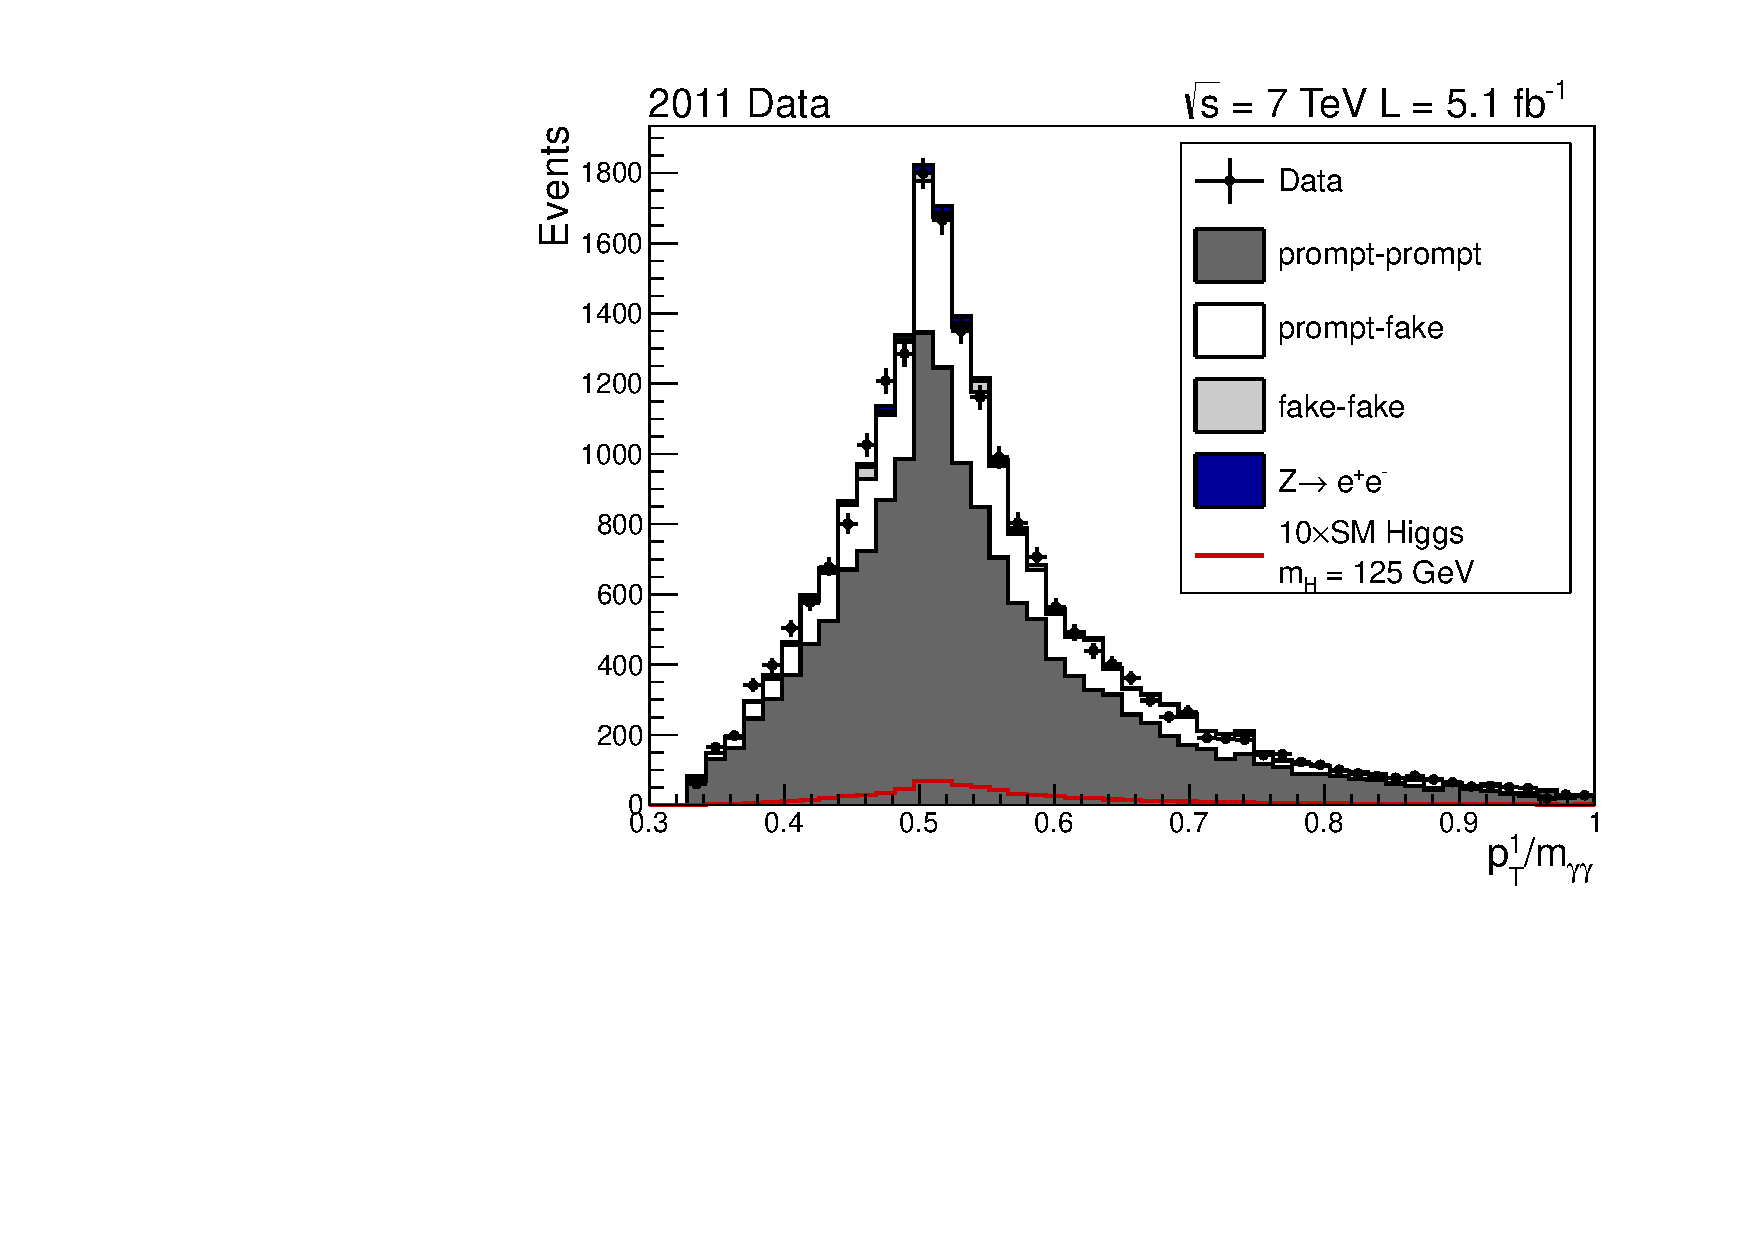
\includegraphics[width=0.48\textwidth]{hgg7TeV/variablePlots/pt_1om}
  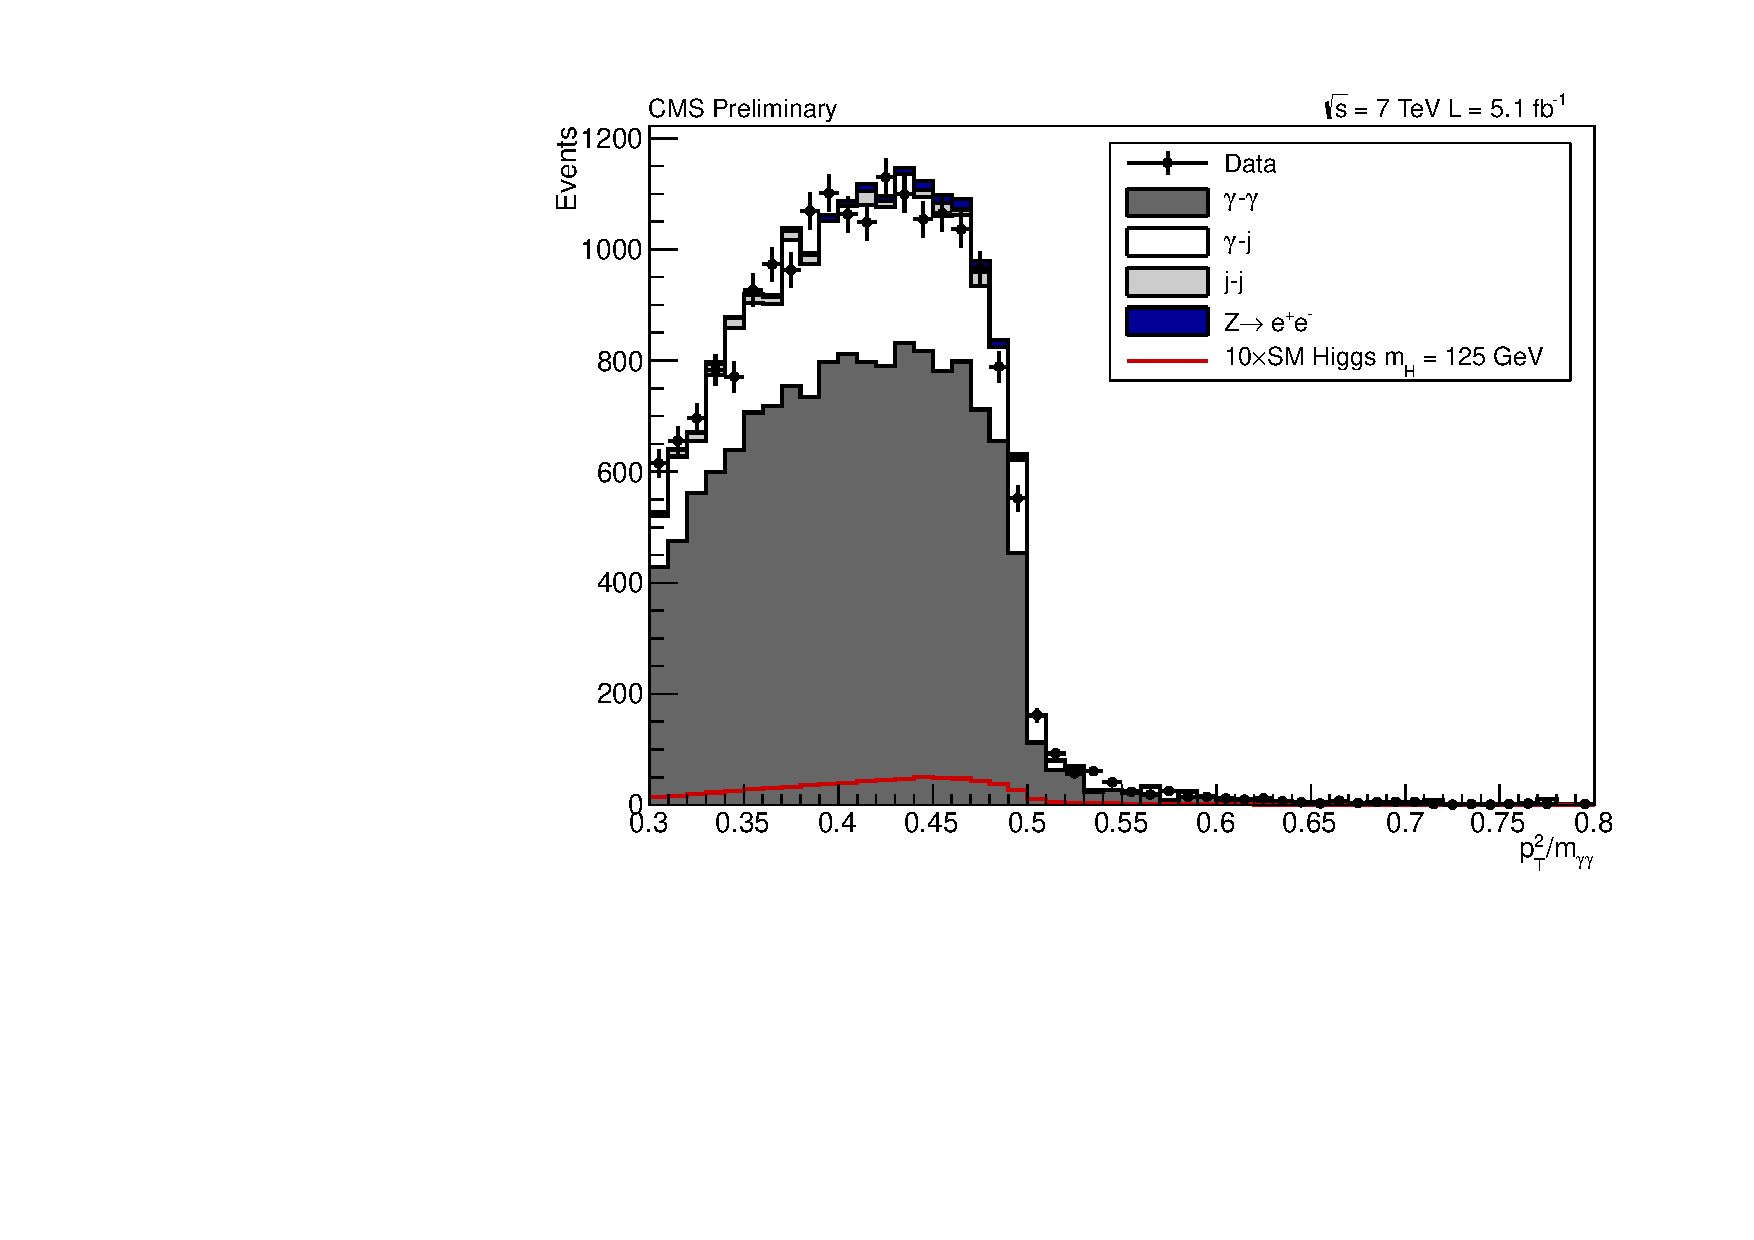
\includegraphics[width=0.48\textwidth]{hgg7TeV/variablePlots/pt_2om}\\
  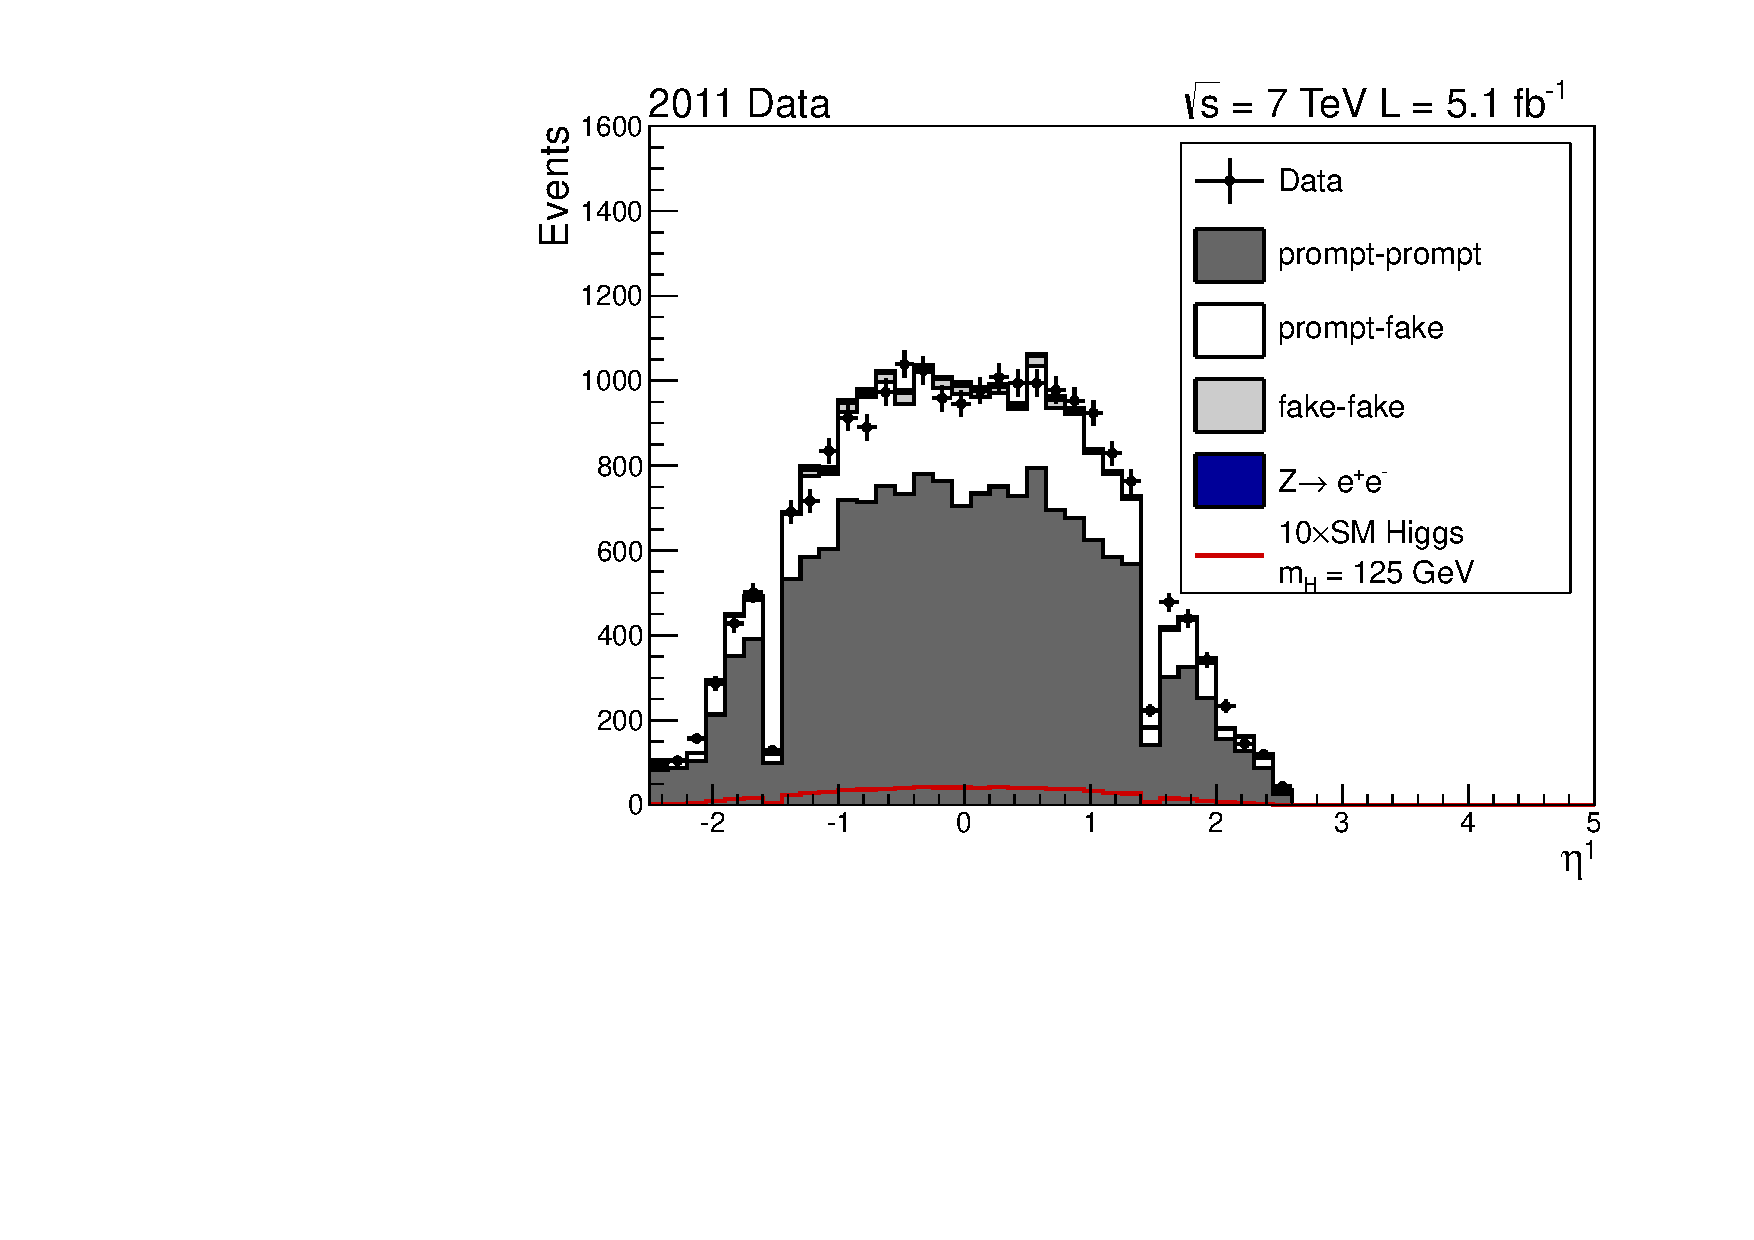
\includegraphics[width=0.48\textwidth]{hgg7TeV/variablePlots/phoeta_1}
  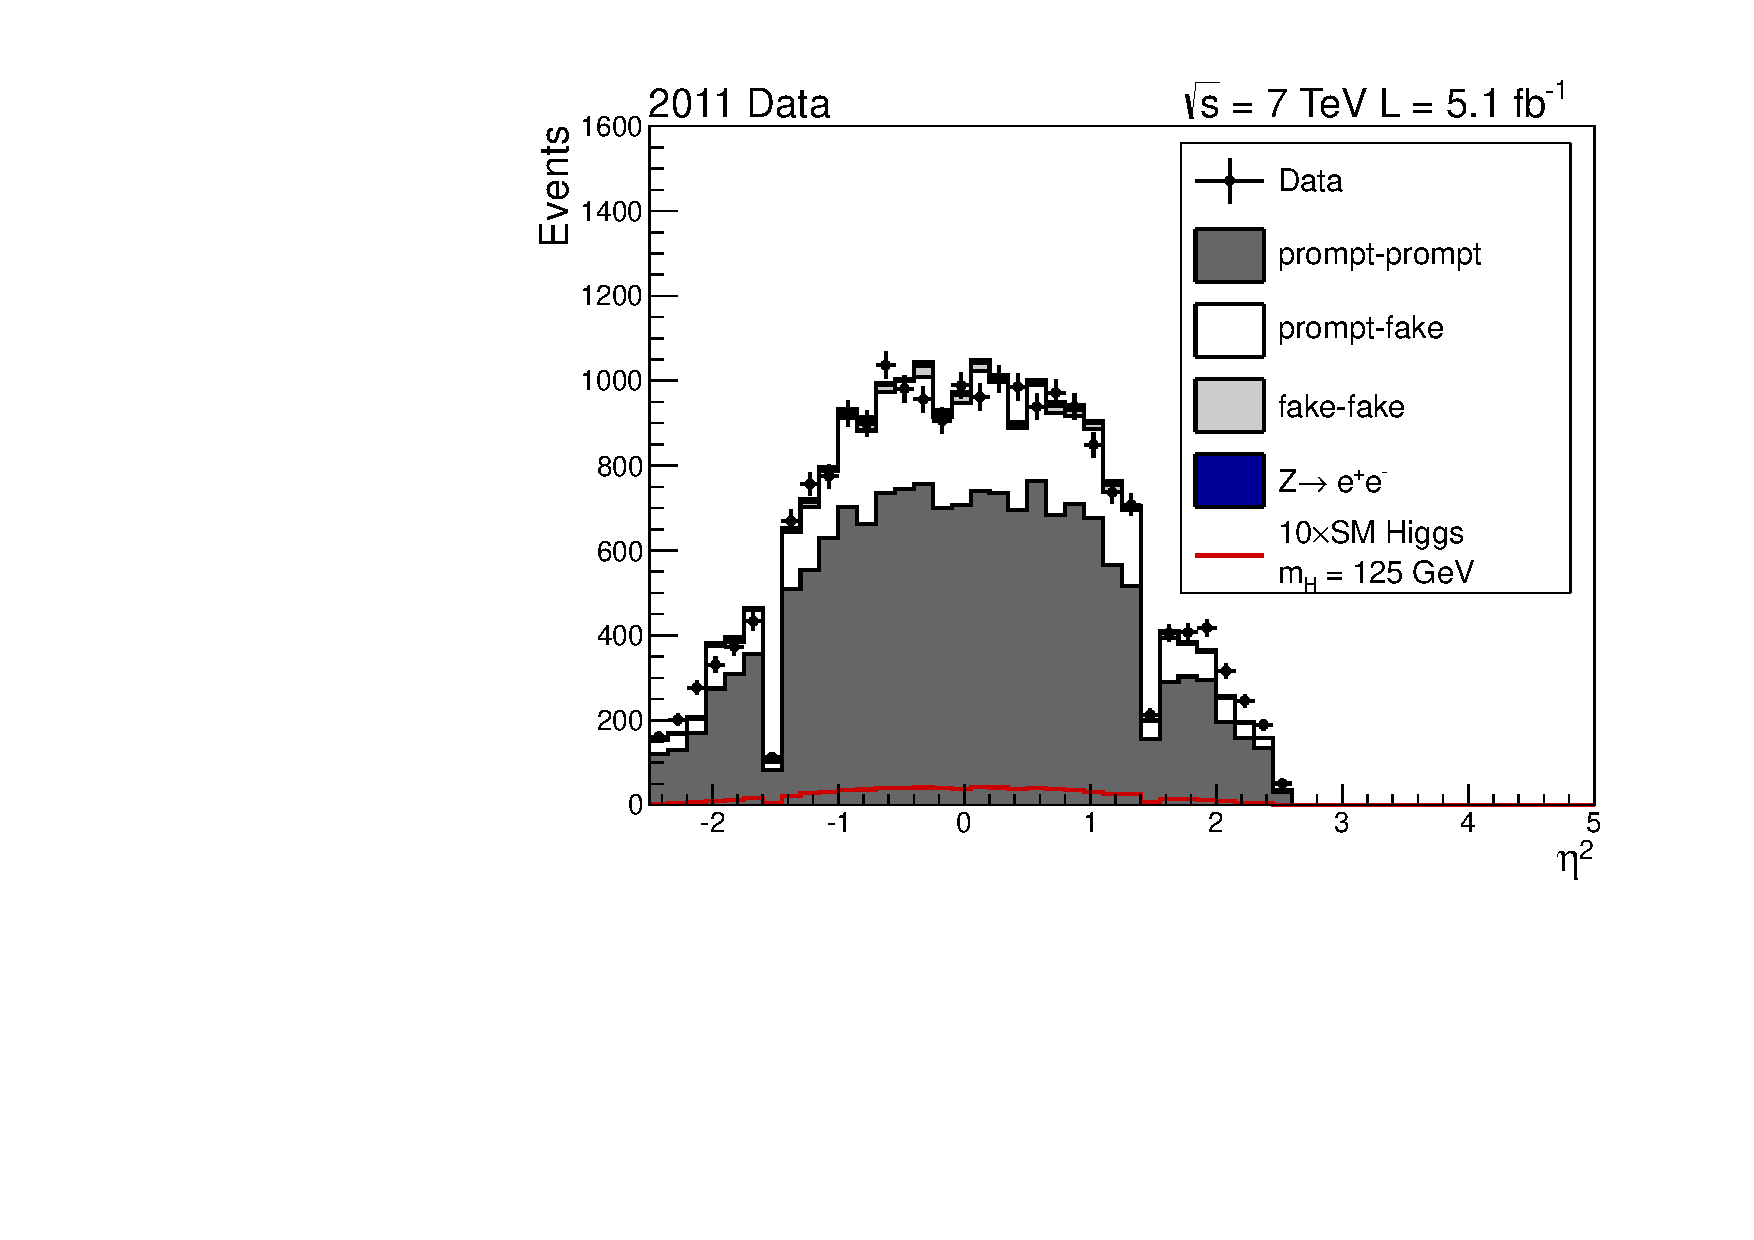
\includegraphics[width=0.48\textwidth]{hgg7TeV/variablePlots/phoeta_2}\\
  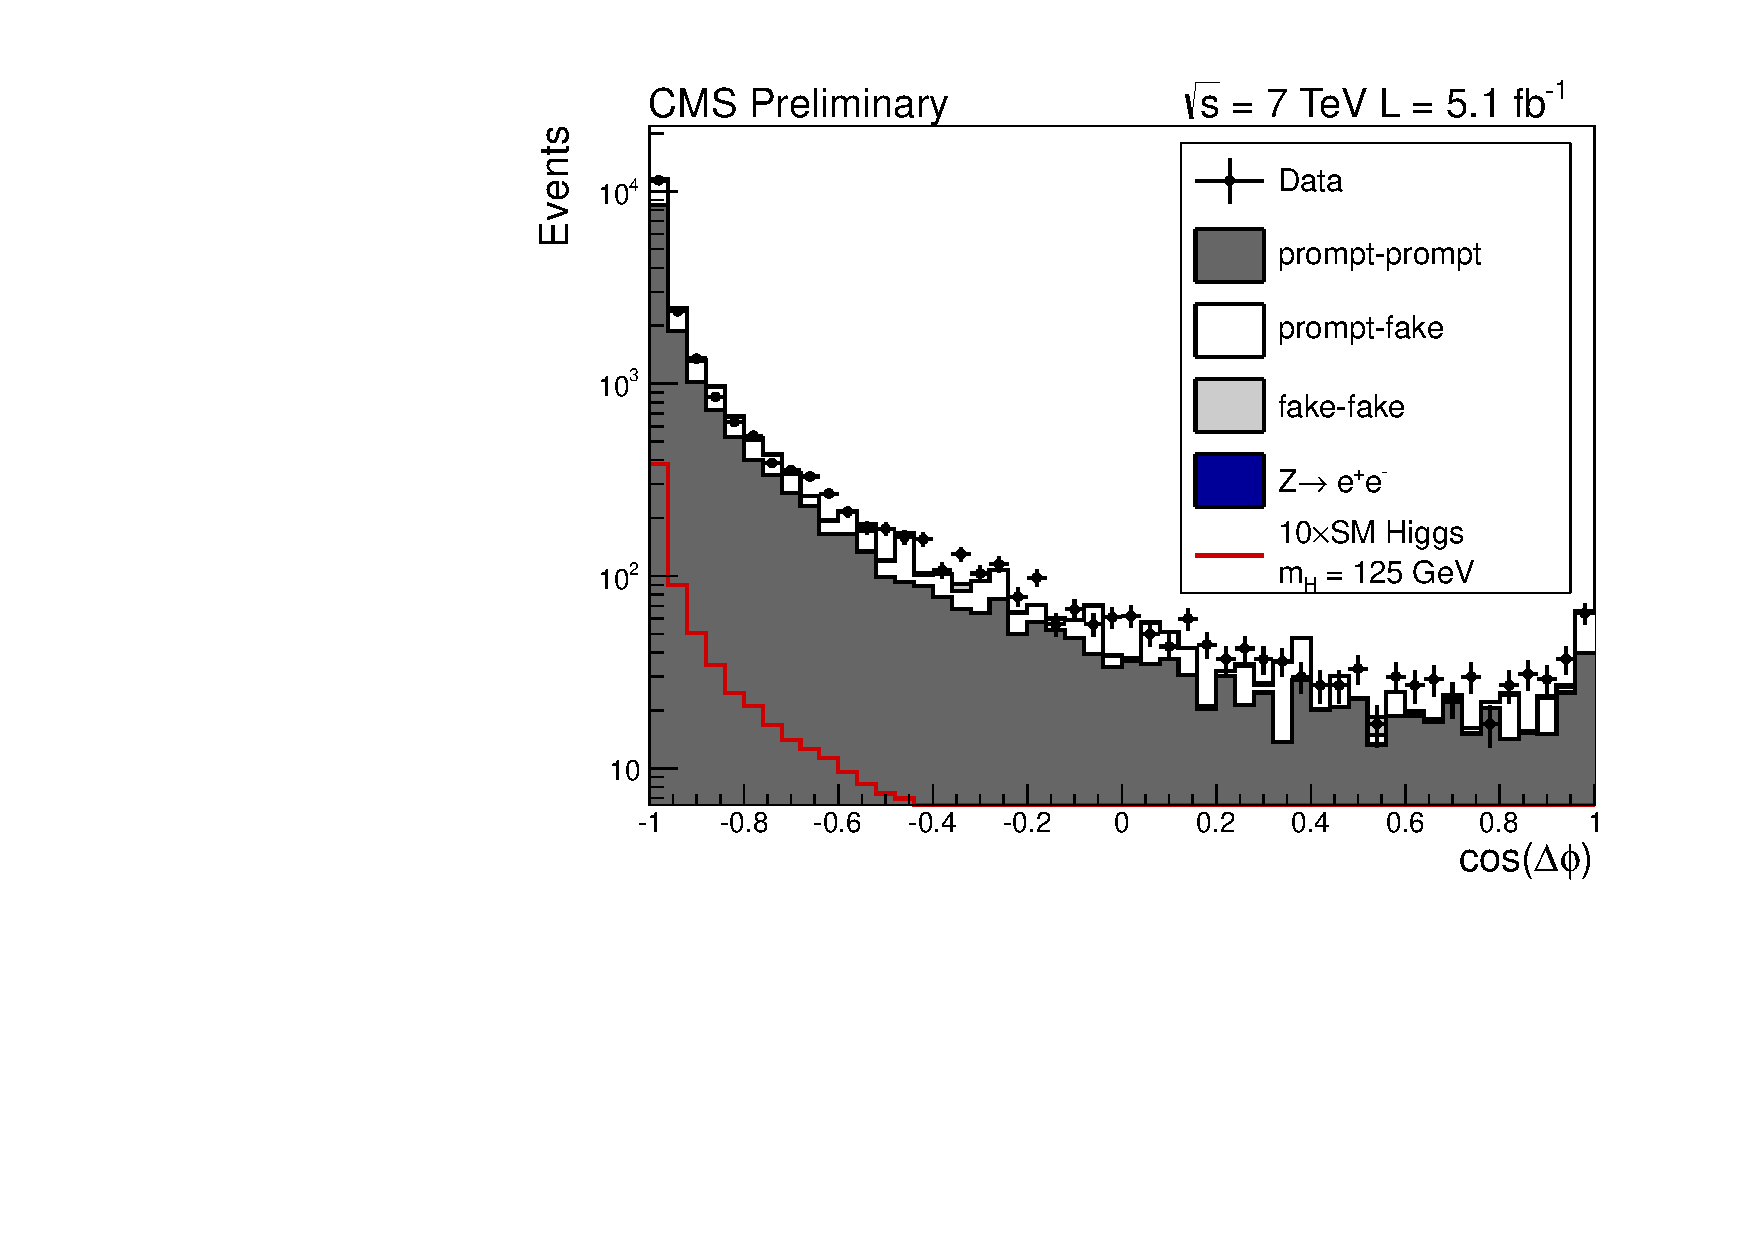
\includegraphics[width=0.48\textwidth]{hgg7TeV/variablePlots/cosdphi}
 \label{fig:diphotonbdtvars1}
 \caption{VARIABLES}
\end{center}
\end{figure}

\begin{figure}[hbt!]
\begin{center}
  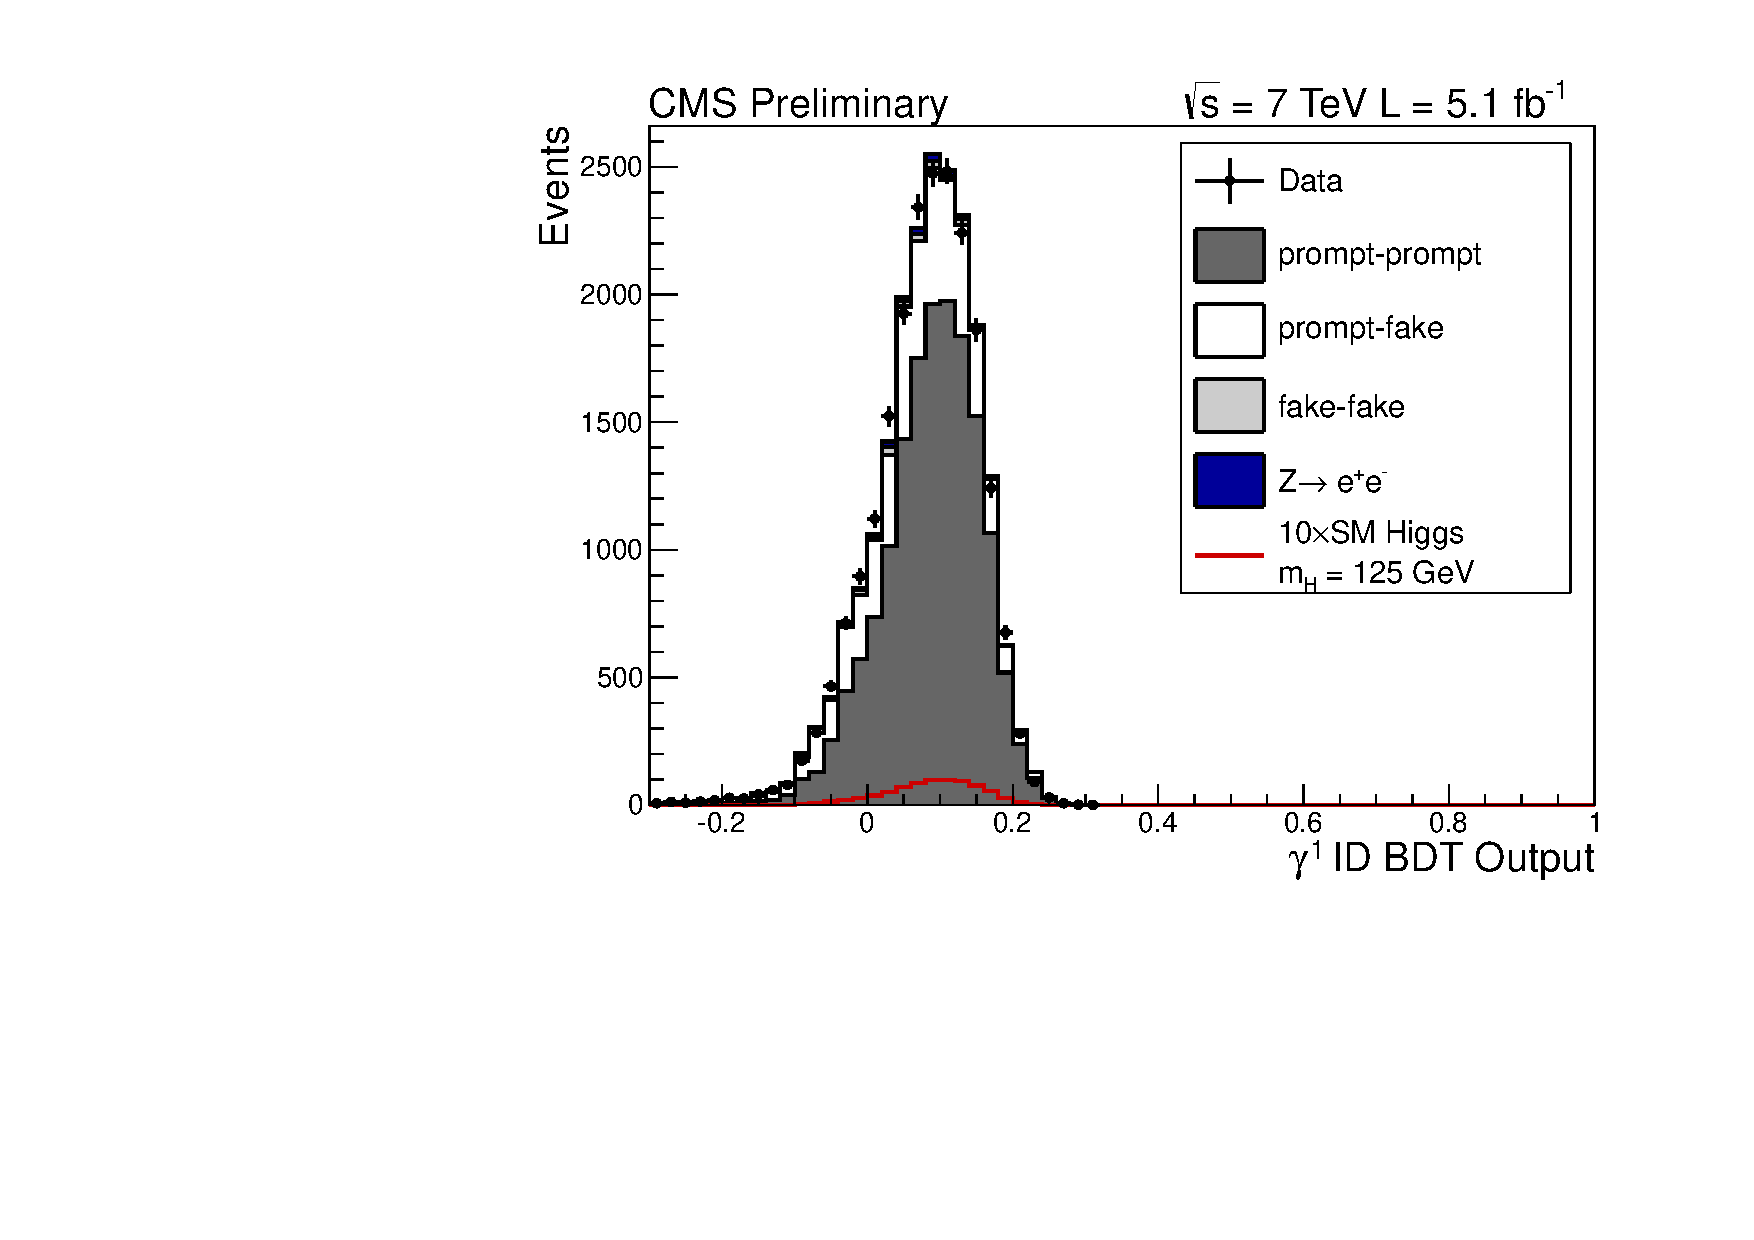
\includegraphics[width=0.48\textwidth]{hgg7TeV/variablePlots/phoid_1}
  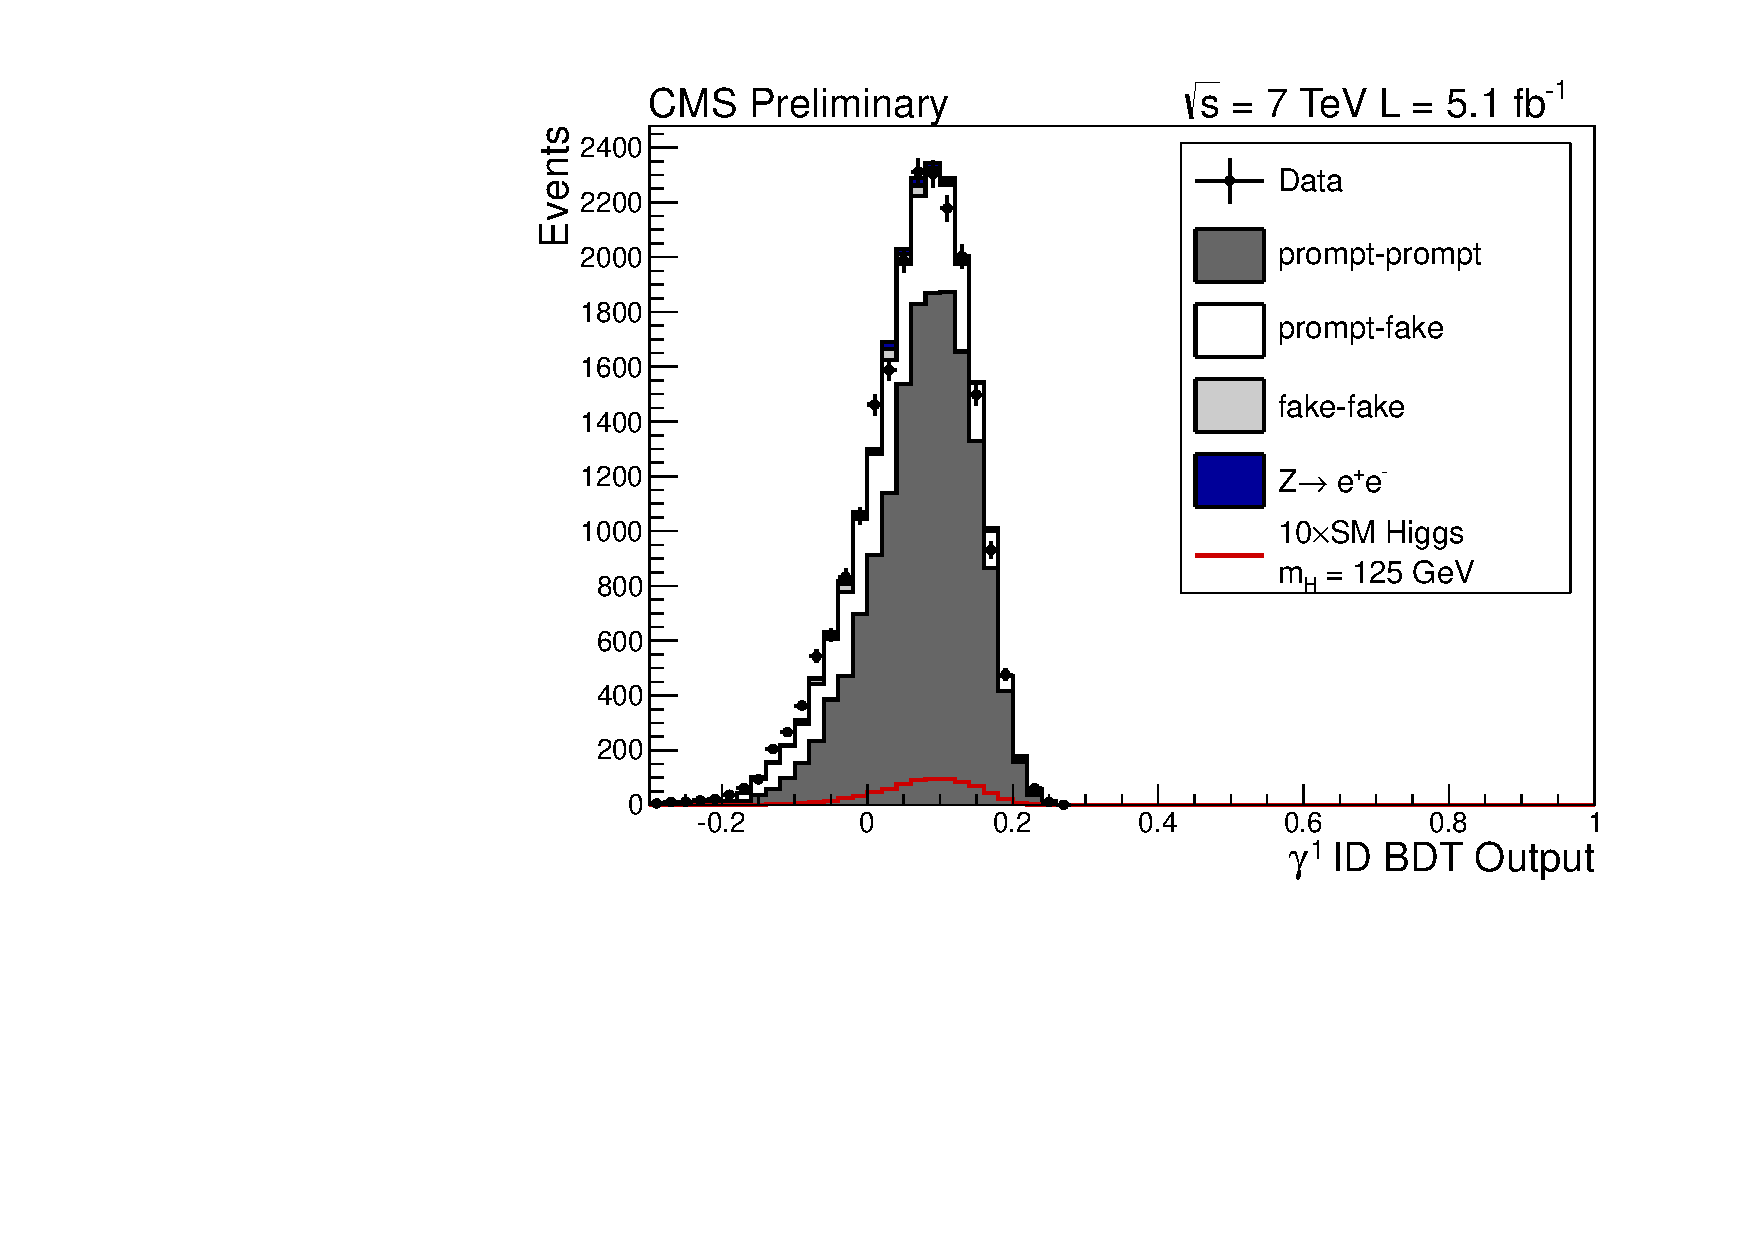
\includegraphics[width=0.48\textwidth]{hgg7TeV/variablePlots/phoid_2}\\
  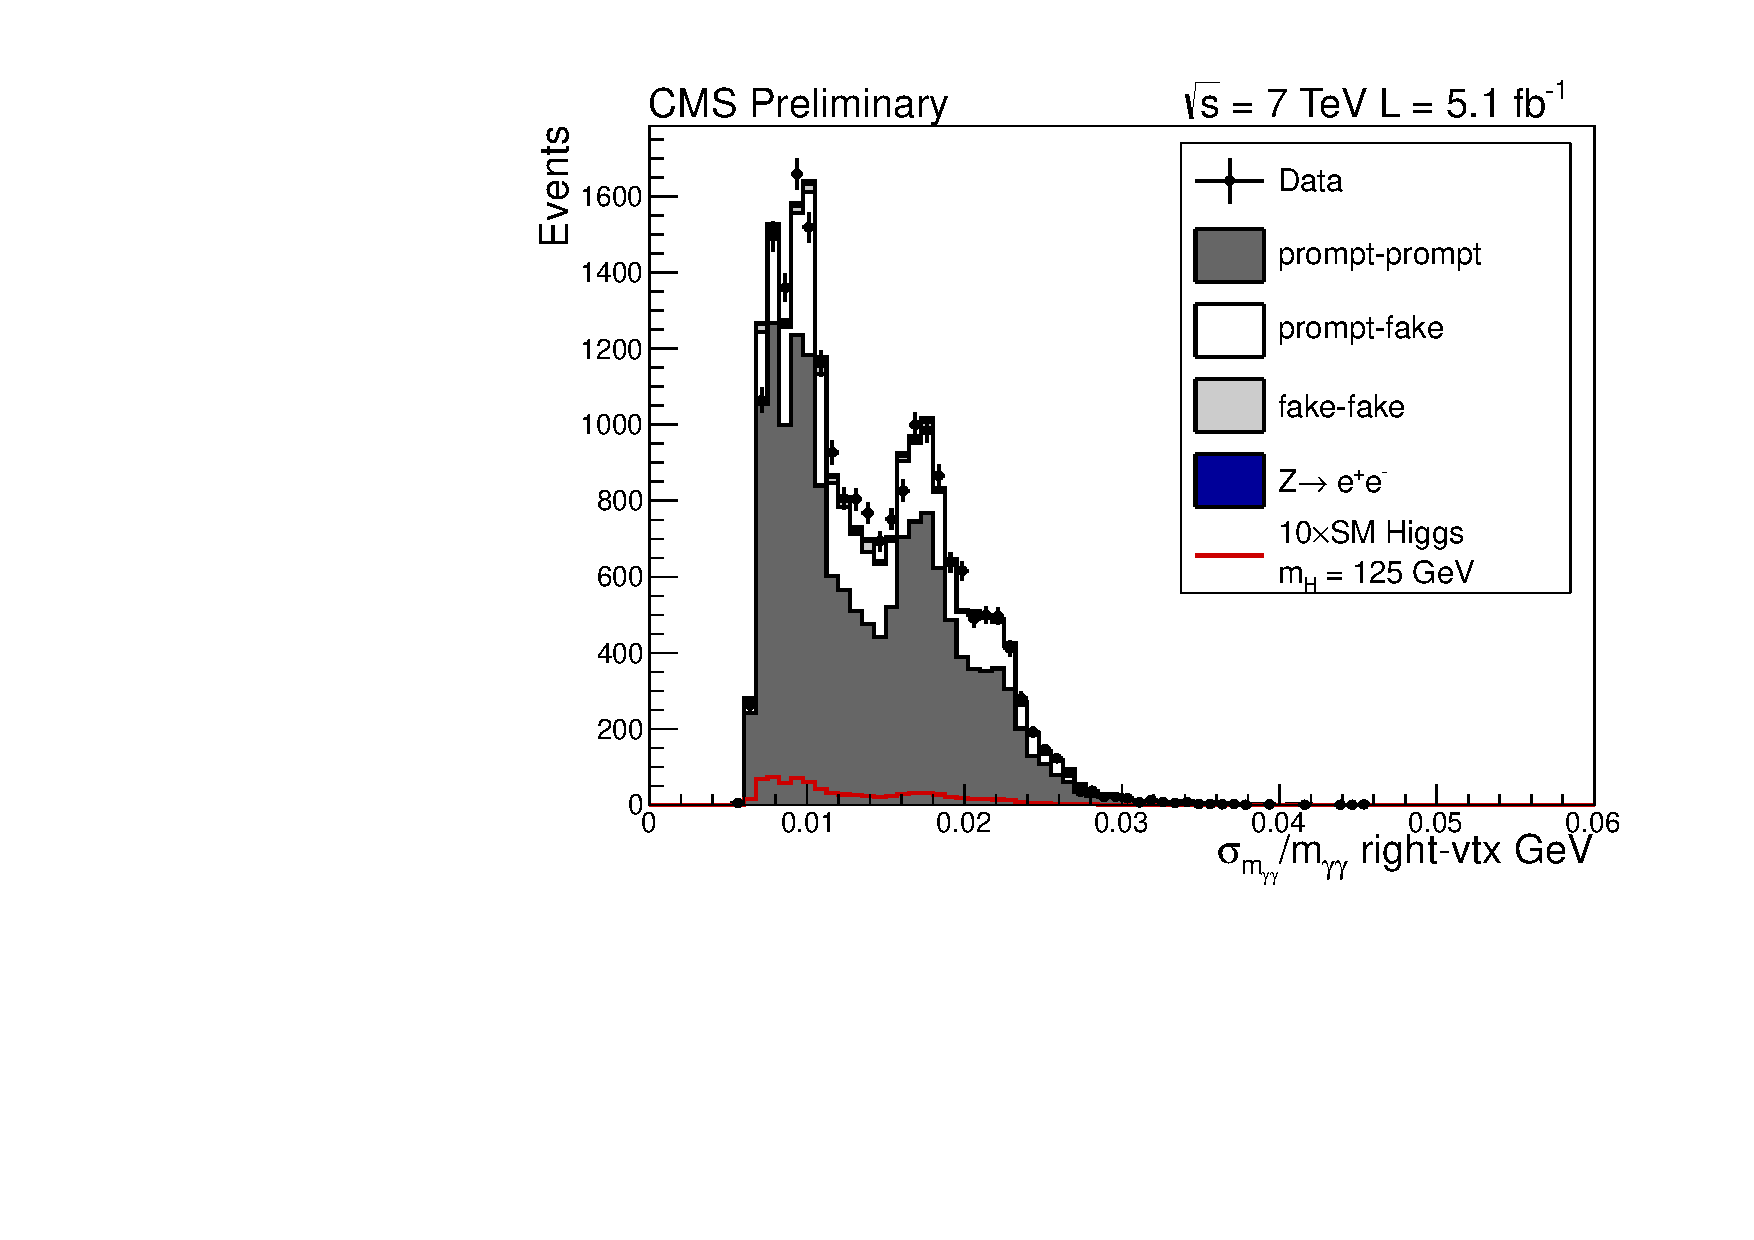
\includegraphics[width=0.48\textwidth]{hgg7TeV/variablePlots/sigmrv}
  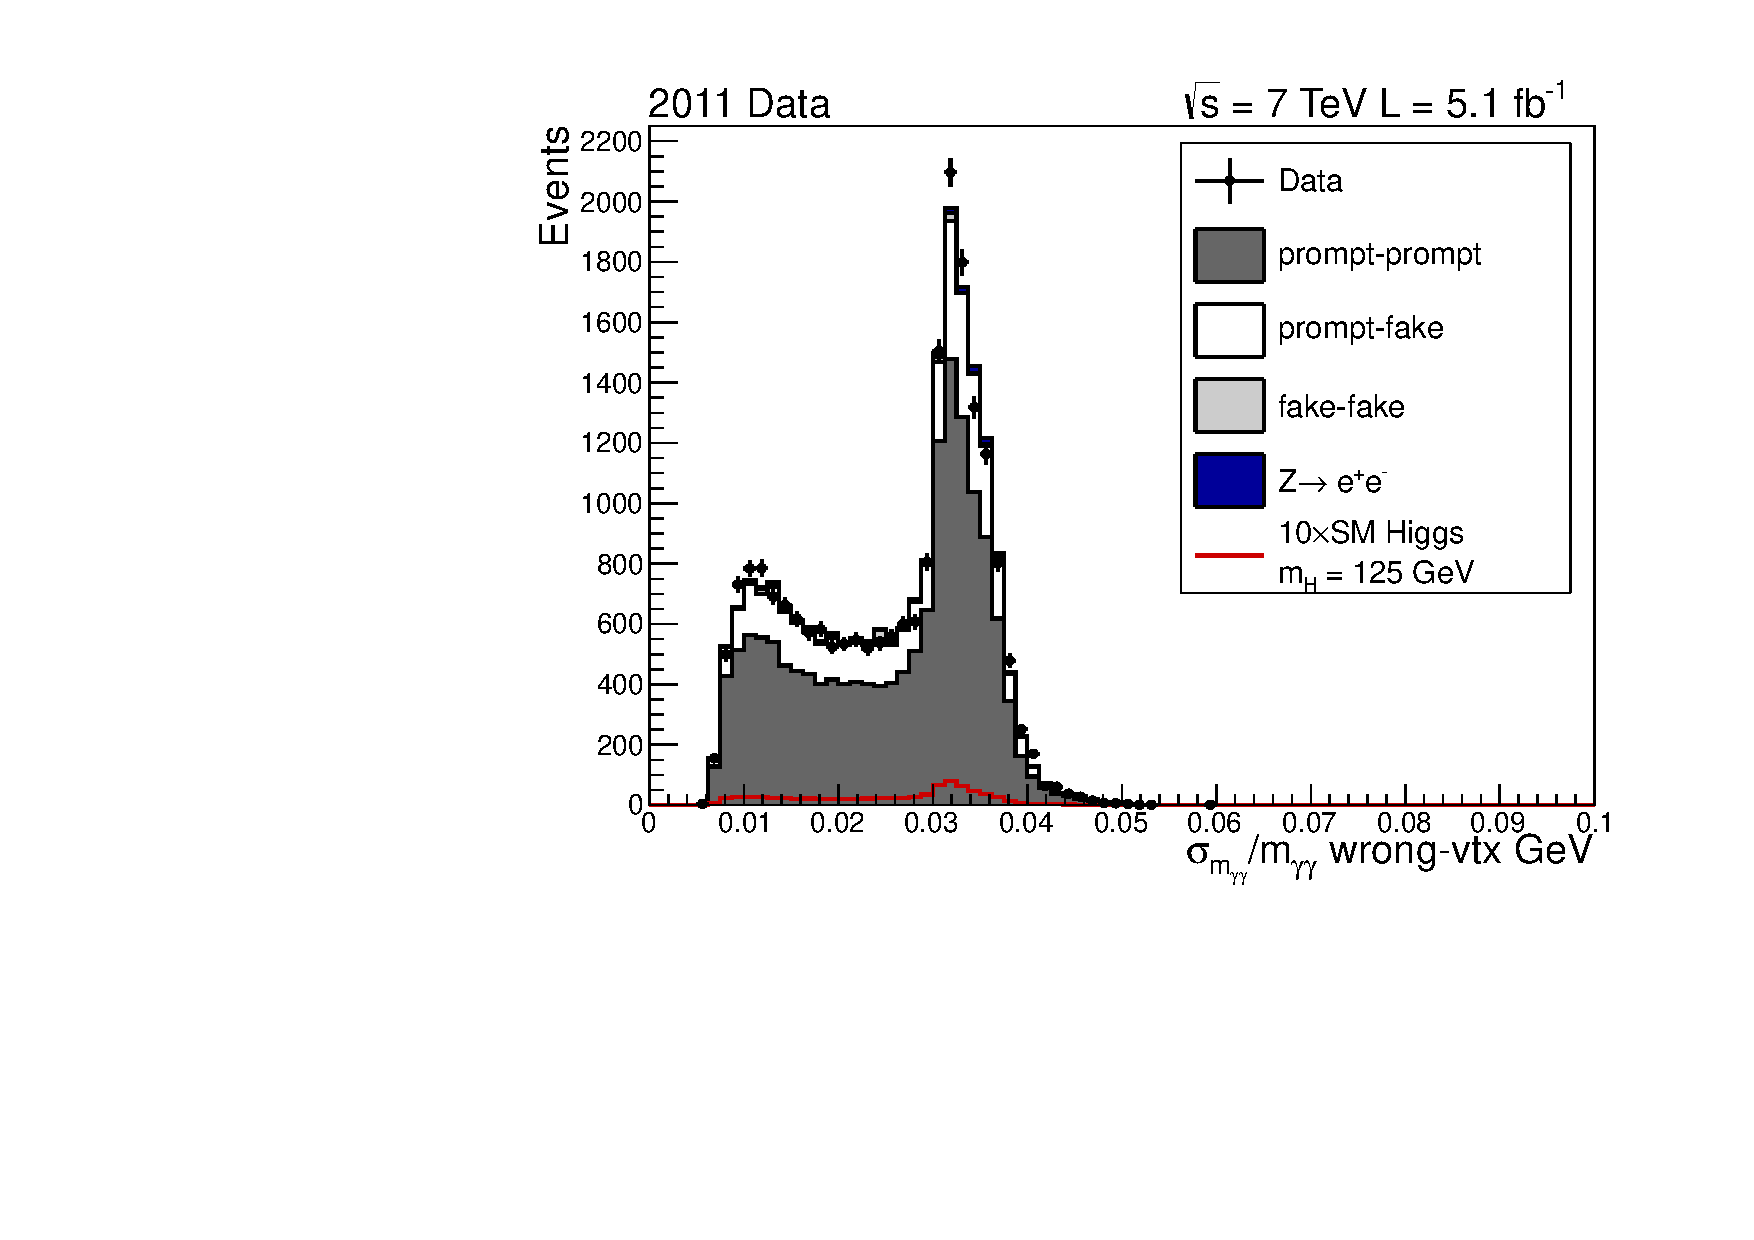
\includegraphics[width=0.48\textwidth]{hgg7TeV/variablePlots/sigmwv}
 \label{fig:diphotonbdtvars2}
 \caption{VARIABLES}
\end{center}
\end{figure}

Figure~\ref{fig:massmcdata} shows the invariant mass distribution in data and MC for events passing the full
selection with a diphoton BDT output greater than 0.05.

\begin{figure}[hbt!]
\begin{center}
  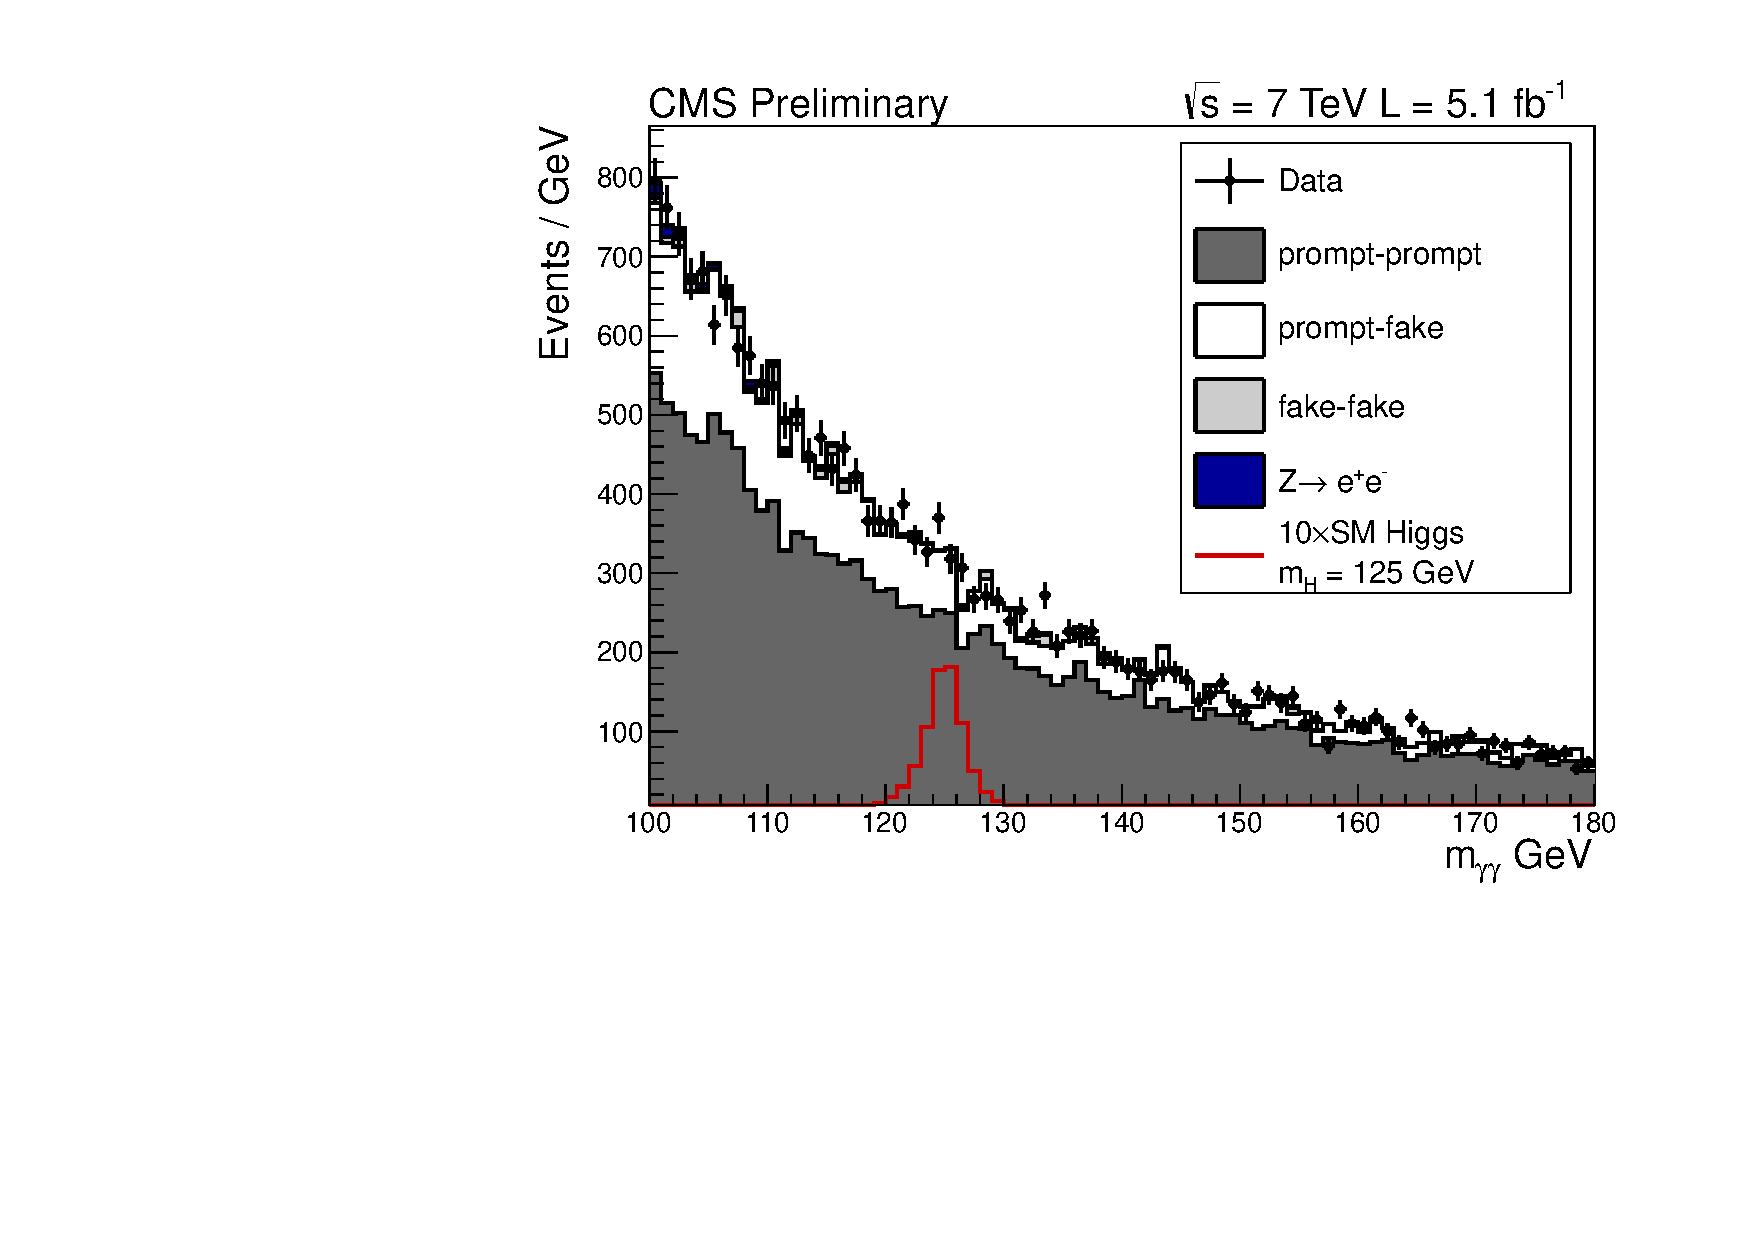
\includegraphics[width=0.5\textwidth]{hgg7TeV/variablePlots/mass}
 \caption{Invariant mass distrobution in data and MC after applying the full event selection in the
 range 100 to 180 GeV. The contribution expected from a SM Higgs with mass 125 GeV, scaled by 10, 
 is shown in red. }
 \label{fig:massmcdata}
\end{center}
\end{figure}


